\documentclass[serif,10pt]{wiley-article}
\bibliographystyle{WileyNJD-AMA}
\usepackage[T1]{fontenc}
\usepackage{subcaption}


\papertype{}
\paperfield{}
\title{Bayesian Inference for Cox Proportional Hazard Models with Partial Likelihoods, Semi-Parametric Covariate Effects and Correlated Observations}


\author[1]{Ziang Zhang}

\author[1,2]{Alex Stringer}

\author[1,2]{Patrick Brown}

\author[1]{James Stafford}



% Include full affiliation details for all authors
\affil[1]{Department of Statistical Sciences, University of Toronto, Ontario,Canada}
\affil[2]{Centre for Global Health Research, St. Michael's Hospital, Ontario,Canada}

\corraddress{Ziang Zhang}
\corremail{aguero.zhang@mail.utoronto.ca}
\fundinginfo{Mr. Stringer is supported by a PGS-D fellowship and Drs Brown and Stafford are supported by Discovery Grants from the Natural Sciences and Engineering Research Council of Canada}


% Include the name of the author that should appear in the running header
\runningauthor{Zhang \textsc{et al}}
\DeclareUnicodeCharacter{2212}{-}
\begin{document}

\begin{frontmatter}
\maketitle

\begin{abstract}
{\fontfamily{ptm}\selectfont
We introduce a novel approximate Bayesian inference methodology for the Cox Proportional Hazard model with partial likelihood, linear covariate effects, semi-parametric covariate effects and correlated survival times. The existing method for approximate Bayesian inference for Cox Proportional Hazard model (Integrated Nested Laplace Approximations, INLA), requires the Hessian matrix of the log-likelihood to be diagonal and is restricted to models with a parametric or smooth semi-parametric baseline hazard. In contrast, the use of partial likelihood in the Cox proportional hazard model does not require assumptions to be made about the baseline hazard, but the Hessian of the log-partial likelihood is fully dense and hence INLA does not accommodate its use. Through the use of quasi-Newton optimization methods, we accommodate the use of a log-likelihood with a dense Hessian in our inference. We hence introduce a novel approximate Bayesian inference methodology for the Cox Proportional Hazard model using its partial likelihood, that allows the inclusion of linear covariate effects, semi-parametric covariate effects and correlated survival times. A simulation study demonstrates the superior accuracy of our method over INLA when the baseline hazard is not smooth. Analysis of a dataset of Leukaemia survival times and a dataset of Kidney infection times demonstrates the use of our method to yield full posterior estimation and uncertainty quantification for the parameters of interest without making smoothness assumptions about the baseline hazard. An R package implementing our method will be released publicly.
}

% Please include a maximum of seven keywords
\keywords{Cox Proportional Hazard Model, Partial Likelihood, Bayesian Inference, Semi-parametric Smoothing}
\end{abstract}
\end{frontmatter}
%\doublespacing
\section{Introduction}\label{sec1}
For problems involving time-to-event data, the combination of Cox proportional hazard (Cox PH) models and inference via partial likelihood has been the dominant methodology following its development by Cox \cite{coxph}. The Cox PH model assumes that any two subjects' event hazards are proportional as a function of time, with the ratio depending on unknown linear or smooth covariate effects which are inferred from the observed data. Event times may be correlated within the sample, for example when the response is time to kidney failure for the left and right kidneys from the same subject. Inference that is conducted via partial likelihood does not require assumptions to be made about the form of the baseline hazard. Further, the use of Bayesian inference with the Cox PH model is desirable as this yields model-based estimation and uncertainty quantification for all parameters of interest. However, existing methods for approximate Bayesian inference based on Integrated Nested Laplace Approximations (INLA) \cite{inla} cannot be applied to the Cox PH model with partial likelihood because the Hessian matrix of the log partial-likelihood is fully dense while INLA requires this matrix to be diagonal. Application of the INLA methodology to the Cox PH model without partial likelihood has been considered \cite{inlacoxph}, but this requires restrictive smoothness assumptions to be made about the baseline hazard.

Recently, Stringer et al. \cite{casecross} developed an approximate Bayesian inference methodology for case-crossover models, which applies the approximation strategy of INLA to a log-partial likelihood with a non-diagonal Hessian matrix. Their methodology includes semi-parametric covariate effects and yields full posterior uncertainty for the corresponding smoothness parameters, an improvement over existing frequentist methods. However, the partial likelihood they consider is simpler than that of the Cox PH model, and the Hessian matrix of their log-partial likelihood is block-diagonal and sparse. In contrast, the Hessian matrix of log-partial likelihood of Cox PH model is fully dense, so the method of Stringer et. al. \cite{casecross} does not apply to this model.

In this paper we extend the approximate Bayesian inference methodology of Stringer et al. \cite{casecross} to the Cox proportional hazard model with partial likelihood. Our methodology accommodates semi-parametric smoothing effects and correlation between observed survival times. We demonstrate improved accuracy over INLA in simulations where the assumption of a smooth baseline hazard is violated. Our point estimates compare favourably to those based on frequentist Generalized Additive Models (GAMs) which use partial likelihood, in cases where INLA does not compare favourably. However, we retain all the advantages of a fully Bayesian approach over GAMs, which includes full posterior uncertainty estimates for all parameters including those related to the smoothness of the covariate effects.

The remainder of this paper is organized as follows. In \S\ref{sec:method}, we describe our proposed methodology and how the quasi-Newton method is used to mitigate the computational problems brought by the dense Hessian matrix. In \S\ref{sec:example} we illustrate our methodology in a simulation study and through the analysis of Leukaemia survival data analysed by Martino et al in 2011 \cite{inlacoxph} and the Kidney catheter data analysed by McGilchrist \cite{kidney} in 1991. We conclude in \S\ref{sec:discussion} with a discussion.


\section{Methods}\label{sec:method}

\subsection{A latent Gaussian Cox PH Model}

Suppose we observe $n$ groups indexed by $i$, each with $n_{i}$ observations indexed by $j$. For example, we may observe $n$ subjects with $n_{i}$ measurements per subject. Denote the random variable representing the $j^{th}$ survival time in the $i^{th}$ group by $T_{ij}$, and denote its realization by $t_{ij}$. Let $c_{ij}$ denote the censoring time for observation $ij$, if $c_{ij} < T_{ij}$, then $T_{ij}$ is not directly observable. The observed time is $y_{ij} = \min\{t_{ij},c_{ij}\}$. Define $d_{ij} = 1$ if $y_{ij} = t_{ij}$ (a survival time) and $d_{ij} = 0$ if $t_{ij} > y_{ij}$ (a censoring time). The observations for each $i,j$ are hence denoted by pairs $y =  \left\{(y_{ij},d_{ij}): i = 1,\ldots,n; j = 1,\ldots,n_{i} \right\}$. The total number of rows in the data set will be denoted by $N = \sum_{i=1}^{n}n_{i}$.

Define $h_{ij}(t)$ to be the hazard function for the random variable $T_{ij}$. The Cox PH model assumes $h_{ij}(t) = h_0(t)\text{exp}(\eta_{ij})$ where $h_0(t)$ is an unknown baseline hazard function that does not depend on the covariates. An additive predictor $\eta_{ij}$ links the covariates for the $ij$th observation to the survival time $T_{ij}$:
\begin{equation}\begin{aligned}\label{eqn:eta}
\eta_{ij} &=x_{ij}^{T}\beta+\sum_{q=1}^{r} \gamma_q(u_{qij}) +\xi_{i} \\
\xi_i &\overset{iid}{\sim} \mathcal{N}(0,\sigma_{\xi}) \\
\gamma_{q}(\cdot) &\overset{ind}{\sim} \mathcal{GP}(\sigma_q)
\end{aligned}\end{equation}
Let $\eta = \left\{ \eta_{ij}: i = 1,\ldots,n; j = 1,\ldots,n_{i}\right\}$ be the vector of all the additive linear predictors. Here $x_{ij}$ is a $p$-dimensional vector of covariates that are modelled as having linear associations with the log-hazard, and $\beta = (\beta_{1},\ldots,\beta_{p})$ are regression coefficients. The $u_{q} = \left\{u_{qij}: i = 1,\ldots,n; j = 1,\ldots,n_{i} \right\}, q = 1,\ldots,r$ are covariate vectors whose association with the log-hazard is modelled semi-parametrically through unknown smooth functions $\gamma_1,\ldots,\gamma_r$. The vector of group intercepts $\xi = \left\{ \xi_{i}: i=1,\ldots,n\right\}$, referred to as ``frailty'' coefficients in the context of survival analysis \cite{frailty}, are included to model correlation between survival times coming from the same group $i$. There is no global intercept $\beta_{0}$ as this would be absorbed by $h_{0}(t)$.

\subsection{Modelling Smooth functions}\label{subsec:smooth}
The smooth functions $\gamma_q$ are Gaussian processes, each with a standard deviation parameter $\sigma_q$. A typical choice
for the Gaussian process is the random walk of order 2 \cite{rw2}, which has similarities with cubic spline functions.
The model above is a Latent Gaussian Model (LGM), as $\xi_i$ and $\gamma_q$ are normally distributed and a Normal
prior is specified for the regression coefficients $\beta$. The Gaussian assumption for $\xi_i$ and $\gamma_q$ is essential for the inference methodology in the next section.

Let $U_{q} = \{U_{ql};l = 1, ...., m_q\}$ be the ordered vector of distinct values of covariate $u_q,q = 1,\ldots,r$; often these values are set by the user by discretizing the covariate $u_q$ into $m_q$ pre-specifed bins. To infer the infinite-dimensional parameters $\gamma_{q},q = 1,\ldots,r$, we approximate each by a piecewise constant function with jumps at the $U_{ql}$, which we denote as $\gamma_{q}(U_{ql}) = \Gamma_{ql}$. We define the vectors of function values $\Gamma_{q} = \left\{ \Gamma_{q1},\ldots,\Gamma_{qm_{q}}\right\}$ and these are have Gaussian distributions $\Gamma_{q}|\sigma_{q}\sim\mathcal{N}\left[ 0,\Sigma_{q}(\sigma_{q})\right]$ for each $q = 1,\ldots,m_{q}$. These distributions are parametrized through their precision matrices $\Sigma_{q}(\sigma_{q})$ corresponding to the specific Gaussian processes chosen, which depend on parameters $\sigma_{q}$. We define $\Gamma = (\Gamma_{1},\ldots,\Gamma_{r})$ and write $\Gamma|\sigma_{1},\ldots,\sigma_{q}\sim\mathcal{N}\left( 0,\Sigma^{-1}_{\Gamma}\right)$ with $\Sigma^{-1}_{\Gamma} = \text{diag}\left[ \Sigma_{1}^{-1}(\sigma_{1}),\ldots,\Sigma_{r}^{-1}(\sigma_{r})\right]$.

These models usually contain an intercept $\beta_{0}$ and a \emph{sum-to-zero} constraint $\sum_{q=1}^{r}\Gamma_{q} = 0$, for identifiability of parameters. However, $\beta_{0}$ is not identifiable when using the partial likelihood for inference, and hence the sum-to-zero constraint is difficult to interpret in this setting. We fit the following modified RW2 model for each $q = 1,\ldots,r$:
\begin{equation}\begin{aligned}\label{eqn:rw2}
\Gamma_{q,l+1} - 2\Gamma_{q,l} + \Gamma_{q,l-1} &\overset{iid}{\sim}\text{N}\left( 0,\sigma^{2}_{q}\right), \\
\Gamma_{q,a} = 0,
\end{aligned}\end{equation}
where $a\in\left\lbrace 1,\ldots,m_{q}\right\rbrace$ is some chosen reference value. This parametrization is identifiable under the partial likelihood and gives a clear interpretation of $\Gamma_{q,l}$ as the change in log-risk for an individual with covariate value $u_{q,l}$ compared to an individual with covariate value $u_{q,a}$. 

Finally, define the variance parameter vector $\theta = (\theta_{0},\ldots,\theta_{r})$ where $\theta_{q} = -2\log\sigma_{q},q = 1,\ldots,r$, and $\theta_{0} = -2\log\sigma_{\xi}$. The variance parameters are given prior distribution $\theta \sim \pi(\theta)$. 

\subsection{Approximate Bayesian Inference}

Inference is carried out via a partial likelihood function. Define the \textit{risk set} $R_{ij} = \left\{k,l : y_{kl} \geq y_{ij}\right\}$. Assuming $y_{ij} \neq y_{kl}$ when $(i,j) \neq (k,l)$, the partial likelihood can be written as follows: 
\begin{equation}\begin{aligned}\label{eqn:partial}
\pi(y|\eta) &= \prod_{i=1}^{n}\prod_{j=1}^{n_{i}} \bigg\{\frac{\exp[\eta_{ij}]}{{\sum_{l,k\in R_{ij}}^{}\exp[\eta_{lk}]}}\bigg \}^{d_{ij}} \\
&= \prod_{i=1}^{n}\prod_{j=1}^{n_{i}} \bigg\{\frac{1}{{1 + \sum_{l,k\in R_{ij} , (l,k) \neq (i,j)}\exp[\Delta_{lk,ij}]}}\bigg \}^{d_{ij}} \\
\end{aligned}\end{equation}
where $\Delta_{lk,ij} = \eta_{lk} - \eta_{ij}$. Ties in survival times are handled according to the method of Breslow \cite{Breslow}. Note that $h_{0}(t)$ does not appear in the partial likelihood, and hence inference may be carried out in the absence of assumptions about $h_{0}(t)$. Also note that this partial likelihood can be written in the following form:
\begin{equation}\begin{aligned}\label{eqn:whyINLAfail1}
\pi(y|\eta) &= \prod_{i=1}^{n}\prod_{j=1}^{n_{i}} \pi(y_{ij}|\eta)
\end{aligned}\end{equation}
while in order for a model to be compatible with INLA, its likelihood must have the form:
\begin{equation}\begin{aligned}\label{eqn:whyINLAfail2}
\pi(y|\eta) &= \prod_{i=1}^{n}\prod_{j=1}^{n_{i}} \pi(y_{ji}|\eta_{ij}),
\end{aligned}\end{equation}
Martino et al. \cite{inlacoxph} are able to write the likelihood for their Cox PH model in the form (\ref{eqn:whyINLAfail2}) using the full, not partial likelihood (\ref{eqn:partial}). Because of this, they require assumptions to be made about the baseline hazard.

For computational purposes, we follow Rue et al. \cite{inla} and Stringer et al. \cite{casecross} to add a small random noise on the additive predictor, redefining: 
\begin{equation}\begin{aligned}\label{eqn:etaredefine}
\eta_{ij} =x_{ij}^{T}\beta+\sum_{q=1}^{r} \gamma_q(u_{q_{ij}}) +\xi_{i} + \epsilon_{ij}
\end{aligned}\end{equation}
where $\epsilon_{ij} \stackrel{iid}{\sim} \text{N}(0,\tau^{-1})$ for some large, fixed $\tau$. The addition of these $\epsilon_{ij}$ gives the joint distribution of $\left(\Delta, \Gamma,\beta, \xi \right)$ a non-singular variance matrix. We set $\tau = \exp(7)$ which is well within the broad range of $\exp(2),\ldots,\exp(14)$ which Stringer et. al. \cite{casecross} found to yield very similar inferences and running times. Further redefine $\Delta_{lk,ij} = \eta_{lk} - \eta_{ij}$ in terms of the augmented additive predictors (\ref{eqn:etaredefine}). Note that $\Delta_{lk,ij} = \Delta_{11,ij} - \Delta_{11,lk}$ for every $(i,j,l,k)$. To simplify notation, define $\Delta_{ij} = \Delta_{11,ij}$, and note that $\Delta_{11} = 0$. The entire partial likelihood (\ref{eqn:partial}) depends on $\eta$ only through  $\Delta = \left\{\Delta_{ij}: i = 1,\ldots,n; j = 1,\ldots,n_{i} \right\}$. For the remainder of the paper we reflect this in our notation, writing $\pi(y|\Delta) \equiv \pi(y|\eta)$ and defining the log-likelihood $\ell(\Delta; y) = \log\pi(y|\Delta)$.

Define $W = \left(\Delta, \Gamma,\beta, \xi \right)$ which we refer to as the \textit{latent parameters} and let $\text{dim}(W) = m$. Our model specifies $W|\theta\sim\text{N}\left[ 0,Q^{-1}_{\theta}\right]$. An expression for $Q_{\theta}$ is given in \S\ref{sec:method} and a derivation is given in Appendix A. Our main inferential interest is to obtain the marginal posterior distributions of the latent parameters:
\begin{equation}\begin{aligned}\label{eqn:interestedQuat3}
\pi(W_{s}|y) = \int \pi(W_{s}|y,\theta) \pi(\theta|y) d\theta, s = 1,\ldots,m  \\
\end{aligned}\end{equation}
These are used for point estimates and uncertainty quantification of the latent parameters, which often include the effects of primary interest. We are also interested in the joint posterior distributions of the variance parameters:
\begin{equation}\begin{aligned}\label{eqn:interestedQuat1}
\pi(\theta|y) = \frac{\int \pi(W,y,\theta) dW}{\int_{} \int_{} \pi(W,y,\theta) dW d\theta } \\
\end{aligned}\end{equation}
These are used for point estimates and uncertainty quantification of the variance parameter $\theta$, and appear as integration weights in (\ref{eqn:interestedQuat3}). Of secondary inference is the joint posterior distribution of the latent parameters:
\begin{equation}\begin{aligned}\label{eqn:interestedQuat2}
\pi(W|y) = \int \pi(W|y,\theta) \pi(\theta|y) d\theta  \\
\end{aligned}\end{equation}
This appears primarily as an intermediate step in the calculation of the marginal posteriors (\ref{eqn:interestedQuat3}).

All of the quantities of interest (\ref{eqn:interestedQuat3}) -- (\ref{eqn:interestedQuat2}) depend on intractable high-dimensional integrals. Stringer et al. \cite{casecross} utilize Gaussian and Laplace approximations combined with numerical quadrature to approximate each of these integrals accurately and efficiently. Their approximations take the form:
\begin{equation}\begin{aligned}\label{eqn:integration}
\tilde{\pi}(W_{s}|y) &= \sum_{k=1}^{K}
\tilde{\pi}_{G}(W_{s}|y,\theta^{k})
\tilde{\pi}_{LA}(\theta^{k}|y)\delta_{k}, s = 1,\ldots,m \\
\tilde{\pi}(W|y) &= \sum_{k=1}^{K}
\tilde{\pi}_{G}(W|y,\theta^{k})
\tilde{\pi}_{LA}(\theta^{k}|y)\delta_{k} \\
\end{aligned}\end{equation}
where $\left\{\theta^{k},\delta_{k}\right\}_{k=1}^{K}$ is a set of nodes and weights corresponding to an appropriate numerical quadrature rule. The $\tilde{\pi}_{G}(W_{s}|y,\theta^{k})$ is a Gaussian approximation for $\pi(W_{s}|y,\theta^{k})$ and the $\tilde{\pi}_{LA}(\theta^{k}|y)$ is a Laplace approximation for $\pi(\theta^{k}|y)$, which we describe at below.

The approximations (\ref{eqn:integration}) are computed as follows. For any fixed $\theta$, define
\begin{equation}\begin{aligned}\label{eqn:modeandhessian}
\widehat{W}_{\theta} = \left( \widehat{\Delta}_{\theta},\widehat{\Gamma}_{\theta},\widehat{\beta},\widehat{\xi}_{\theta}\right) &= \text{argmax}_{W}\log\pi(W|\theta,y) \\ 
H_{\theta}(W) &= -\frac{\partial^{2}}{\partial W \partial W^{T}}\log\pi(W|\theta,y) \\
v_{\theta,s}^{2} &= \left[H_\theta \left(\widehat{W}_{\theta}\right) ^ {-1} \right]_{ss}, s = 1,\ldots,m
\end{aligned}\end{equation}
For the conditional posterior
\begin{equation}\begin{aligned}\label{eqn:condpost}
\pi(W|\theta,y) \propto \exp\left\lbrace -\frac{1}{2}W^{T}Q_{\theta}W + \ell\left(\Delta;Y\right)\right\rbrace,
\end{aligned}\end{equation}
a second-order Taylor expansion of $\log(W|\theta,y)$ about $W = \widehat{W}_{\theta}$ yields a Gaussian approximation:
\begin{equation}\label{eqn:gaussianapprox}
\pi(W|\theta,y) \approx \tilde{\pi}_{G}(W|y,\theta) \propto \text{exp}\left\{-\frac{1}{2} \left(W-\widehat{W}_{\theta} \right)^T H_\theta\left(\widehat{W}_{\theta}\right) \left(W-\widehat{W}_{\theta} \right) \right\} \\
\end{equation}
Direct integration of this Gaussian approximation yields a Gaussian approximation for the corresponding marginal density:
\begin{equation}\label{eqb:marginalgaussianapprox}
\tilde{\pi}_{G}(W_{s}|y,\theta) = \int\tilde{\pi}_{G}(W|y,\theta)dW_{-s} \propto\text{exp}\left\{-\frac{1}{2v_{\theta,s}^{2}} \left(W_s-\widehat{W}_{\theta s} \right)^2 \right\}, s = 1,\ldots,m
\end{equation}
For the joint posterior of the variance parameters, the method of Tierney and Kadane \cite{tierney} yields a Laplace approximation:
\begin{equation}\begin{aligned}\label{eqn:laplace}
\pi(\theta|y) \approx \tilde{\pi}_{LA}(\theta|y) \propto \pi(\theta)\left\{\frac{\left|Q_{\theta}\right|}{\left|H_{\theta}\left(\widehat{W}_{\theta}\right)\right|}\right\}^{1/2}\exp\left\{ -\frac{1}{2}\widehat{W}_{\theta}^{T}Q_{\theta}\widehat{W}_{\theta} + \ell\left(\widehat{\Delta}_{\theta};y \right)\right\}
\end{aligned}\end{equation}
The Hessian matrix $H_{\theta}(W)$ has the form $H_{\theta}(W) = Q_{\theta} + C(W)$ where
\begin{equation*}
C(W) = -\frac{\partial^{2}}{\partial W\partial W^{T}}\ell(\Delta) = -\begin{pmatrix}
\frac{\partial^{2}\ell(\Delta;y)}{\partial\Delta\partial\Delta^{T}} & 0 & 0 \\
0 & 0 & 0 \\
0 & 0 & 0 \\
\end{pmatrix}
\end{equation*}
Because the partial likelihood takes the form (\ref{eqn:whyINLAfail1}), $C(W)$ has a dense structure. In contrast, Rue et al. \cite{inla} assume that the likelihood takes the form (\ref{eqn:whyINLAfail2}) which enforces the constraint that $C(W)$ is diagonal and hence their method cannot fit the Cox PH model with partial likelihood. Stringer et al. \cite{casecross} relax this assumption to allow $C(W)$ to have a block-diagonal structure. Our work extends this to permit a fully dense $C(W)$. 

For fixed design matrices $A$, $B$ and $X$, we may write the additive predictor (\ref{eqn:etaredefine}) as:
\begin{equation}
\eta = A\Gamma + B\xi + X\beta + \epsilon
\end{equation}
where $\epsilon \sim \text{N}\left( 0,\tau^{-1}I_{N}\right)$. The partial likelihood (\ref{eqn:partial}) depends on $\eta$ only through $\Delta = D\eta$ where $D$ is an $(N -1) \times N $-dimensional matrix of rank $N -1$. Note that because of this, a global intercept $\beta_{0}$ is not estimable when using partial likelihood. The precision matrix is given by
\begin{equation}\label{eqn:precmat}
Q_{\theta} = \tau\begin{pmatrix}
\Lambda^{-1} & -\Lambda^{-1}DA & -\Lambda^{-1}DB & - \Lambda^{-1}DX \\
- A^{T}D^{T}\Lambda^{-1} & \frac{1}{\tau}\Sigma_{\Gamma}^{-1} +  A^{T}D^{T}\Lambda^{-1}DA &  A^{T}D^{T}\Lambda^{-1}DB &  A^{T}D^{T}\Lambda^{-1}DX \\
- B^{T}D^{T}\Lambda^{-1} &  B^{T}D^{T}\Lambda^{-1}DA & \frac{1}{\tau}\Sigma_{\xi}^{-1} +  B^{T}D^{T}\Lambda^{-1}DB & B^{T}D^{T}\Lambda^{-1}DX \\
- X^{T}D^{T}\Lambda^{-1} &  X^{T}D^{T}\Lambda^{-1}DA & X^{T}D^{T}\Lambda^{-1}DB & \frac{1}{\tau}\Sigma_{\beta}^{-1} +  X^{T}D^{T}\Lambda^{-1}DX \\
\end{pmatrix}
\end{equation}
where $\Lambda = DD^{T}$. Expressions for $D$ and $\Lambda^{-1}$ are given in Appendix A.

\subsection{Optimization method}\label{subsec:opt}

To compute the conditional mode $\hat{W}(\theta)$, we use trust region optimization \cite{trustoptim}. The objective function (\ref{eqn:modeandhessian}) is convex and high-dimensional, and hence trust region methods are well-suited to this problem. The Hessian of the objective function is $H_{\theta}(W) = Q_{\theta} + C(W)$, and hence inherits the dense upper-left bock from $C(W)$. We utilize quasi-Newton updates within each iteration of the trust region optimization, which uses a low-rank approximation to $H_{\theta}(W)$ at each iteration and hence do not require evaluation or storage of this matrix during optimization. While this can increase the number of iterations, the computation loads brought by the dense Hessian matrix are greatly reduced and we are able to perform the optimization (\ref{eqn:modeandhessian}) when $H_{\theta}(W)$ is dense. 

Note that $\widehat{W}_{\theta}$ and $H_{\theta}(\widehat{W}_{\theta})$ are used to compute the approximations (\ref{eqn:integration}) and the associated marginal moments and quantiles and hence the dense $H_{\theta}(\widehat{W}_{\theta})$ needs to be stored after each optimization. The total number of Hessian matrices that needs to be evaluated and stored equals to the number of quadrature points being used for the approximations (\ref{eqn:integration}).



\section{Examples}\label{sec:example}

In this section we present a simulation study and two data analysis examples. Code is available in the online supplementary materials.

\subsection{Simulation study}\label{subsec:sim}

To illustrate the accuracy of our method over INLA when the smoothness assumption for baseline hazard function is violated, we performed a simulation study. We generated $n = 400$ uncorrelated data points from a distribution with baseline hazard $h_{0}(t)$ shown in Figure \ref{fig:simulation} and additive predictor $\eta_{i} = \gamma(u_{i})$ with $\gamma(u) = 1.5 [ \text{sin}(0.8u) + 1 ]$. The covariate is obtained by generating $u_{1},\ldots,u_{n}\overset{iid}{\sim}\text{Unif}(-6,6)$, and discretizing these values into 50 disjoint, evenly-spaced bins. Further, we randomly censored $84$ observations. For the single variance parameter $\sigma$ that controls the smoothness of $\gamma$, we use an Exponential($\lambda$) prior with $\lambda$ chosen such that $\mathbb{P}\left( \sigma > 2.5\right) = 0.5$, which is a penalized complexity prior of Simpson et al.\cite{pcprior}. We fit a RW2 model using our procedure and the R-INLA software \cite{inla}. For the latter we used the default random walk model for the baseline hazard run under its default settings. This implicitly assumes that $h_{0}(t)$ is smooth. In contrast, our procedure does not infer $h_{0}(t)$, and does not make assumptions about its smoothness.

\begin{figure}[ht]
\centering
\subcaptionbox{True baseline hazard function}{
	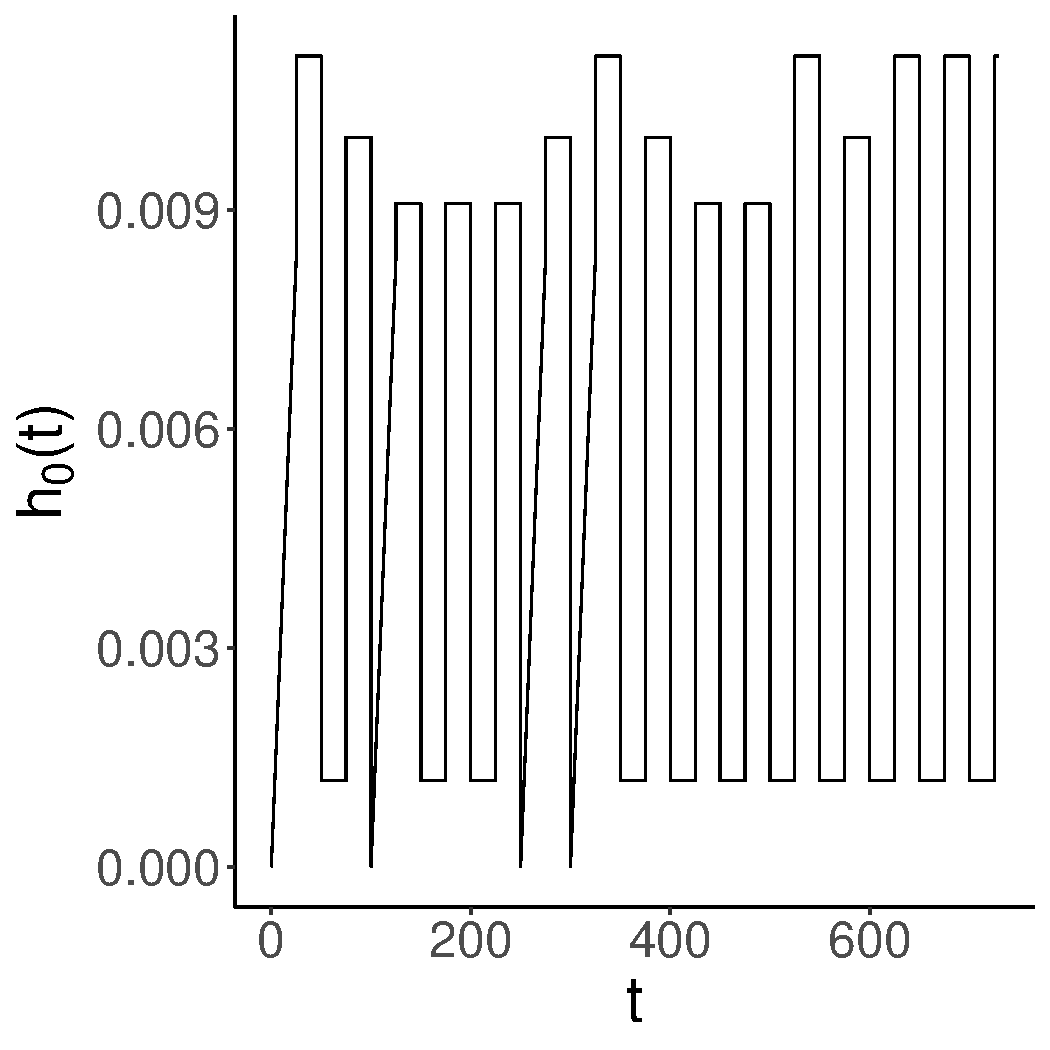
\includegraphics[width=0.45\textwidth,height=3in]{simulation_truebase.pdf}
}
\subcaptionbox{Estimated baseline hazard function (INLA)}{
	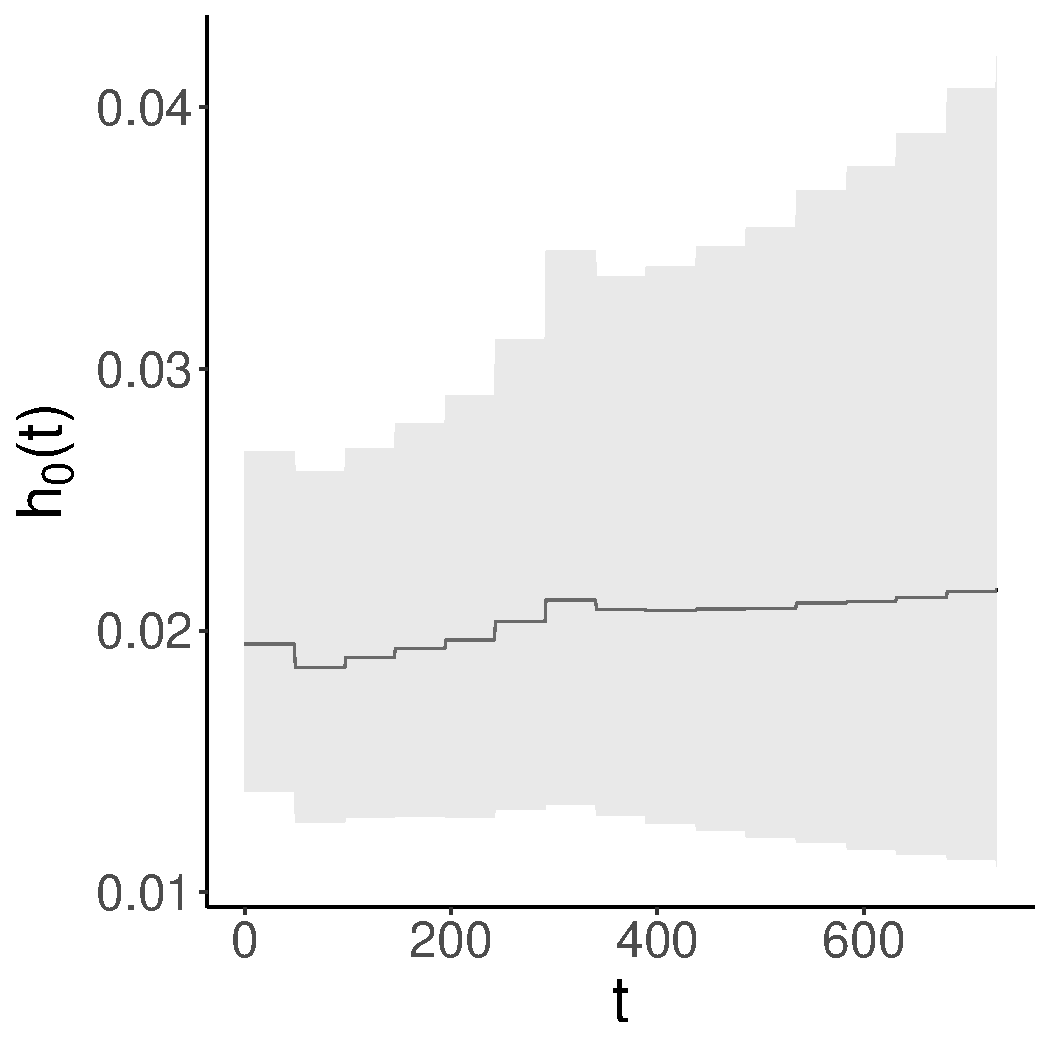
\includegraphics[width=0.45\textwidth,height=3in]{simulation_inlabase.pdf}
}
\subcaptionbox{Posterior estimate of covariate effect}{
	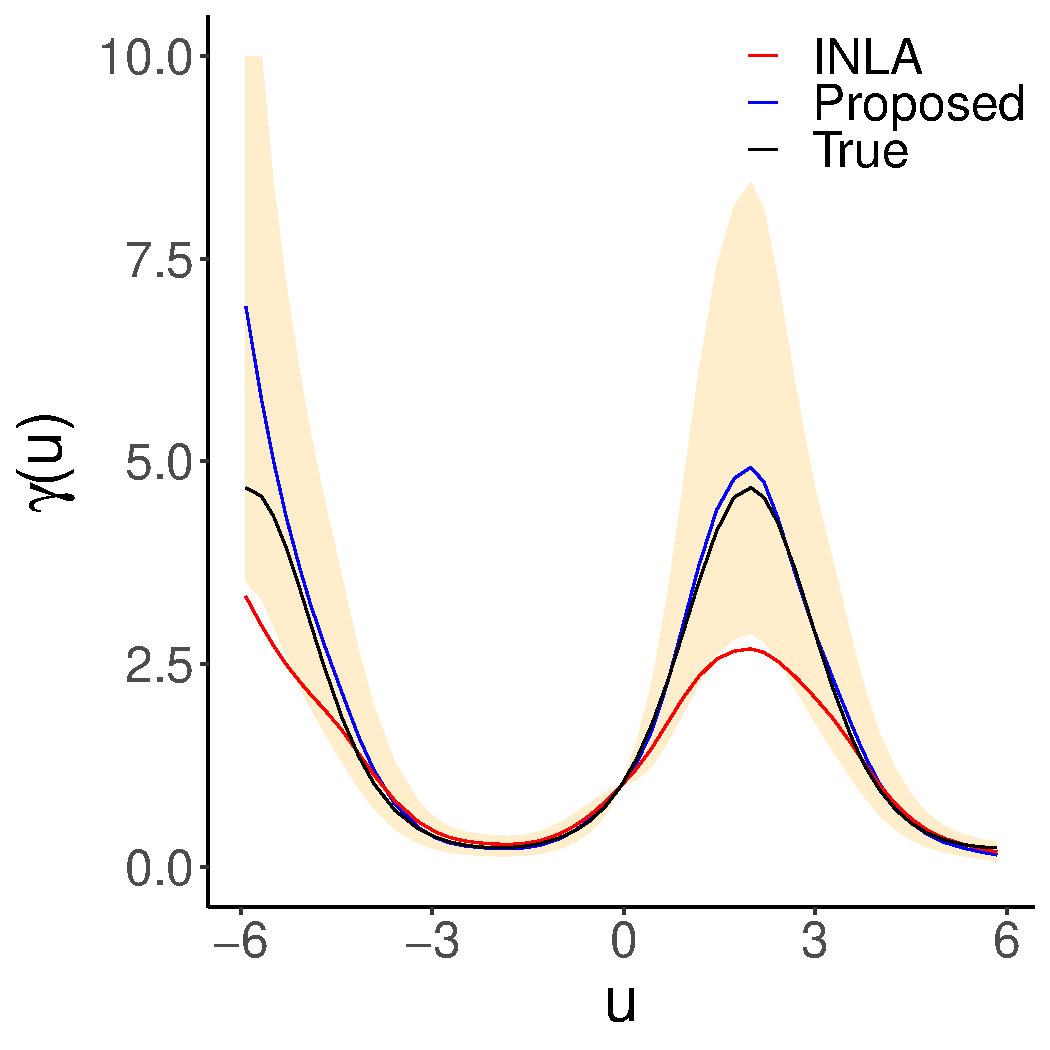
\includegraphics[width=0.45\textwidth,height=3in]{simulation_smooth.pdf}
}
\subcaptionbox{Posterior distribution of $\sigma$}{
	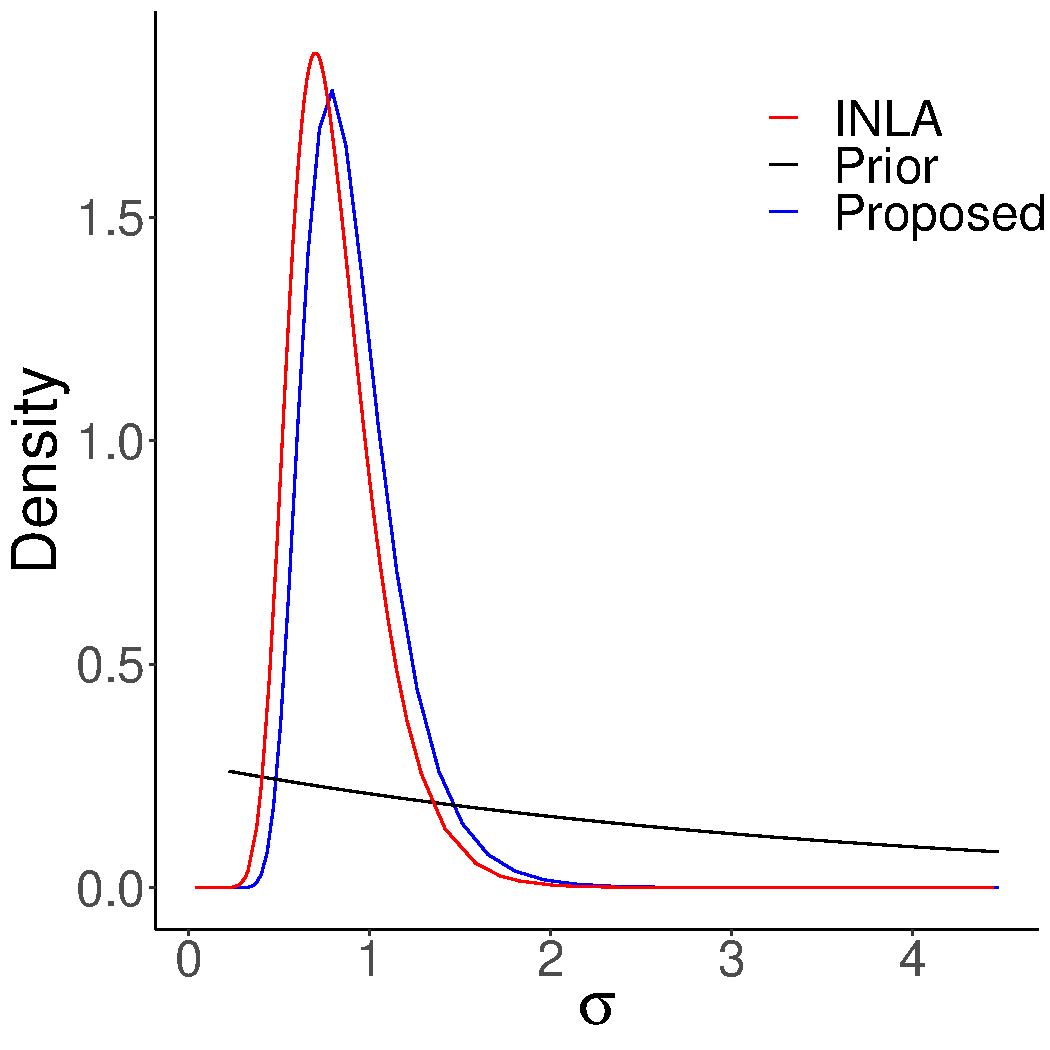
\includegraphics[width=0.45\textwidth,height=3in]{simulation_hyper.pdf}
}
\caption{Results for simulation study in section \ref{subsec:sim}. (a): true baseline hazard function of this simulation. (b): estimated baseline hazard function from INLA and its $95\%$ credible interval(shaded). (c): true risk function (black); posterior mean (blue) and $95\%$ credible interval (shaded) using proposed method; posterior mean using INLA (red). (d): prior (black) and approximate posterior distribution for variance parameter by our method (blue) and by INLA (red).}
\label{fig:simulation}
\end{figure}

Figure \ref{fig:simulation} (a) shows the oscillating baseline hazard, which could represent a scenario where mortality or morbidity risk varies from day to night, or across days of the week, and there are short periods of time where there is no possibility of an event occurring. The inferred baseline hazard from INLA in  Figure \ref{fig:simulation} (b) does not accurately capture the true baseline hazard. The covariate effect in Figure \ref{fig:simulation} (c) is well identified by our partial likelihood analysis, but is severely over-smoothed by INLA.


\subsection{Leukaemia Data}\label{subsec:leuk}

We demonstrate the advantages of our procedure by fitting a semi-parametric Cox PH model to the Leukaemia data set analyzed by Martino et. al. \cite{inlacoxph} The dataset contains information from 1043 independent adult leukaemia patients, with 16 percent of observations right-censored. We are interested in quantifying the relationship between survival rate of leukaemia patients with the age of the patient, the count of white blood cells at diagnosis (wbc), the Townsend deprivation index (tpi) corresponding to the patient's location, and sex of the patient.

The effects of age, sex and white blood cell count were modelled linearly. The deprivation index was discretized into 50 equally spaced bins and modelled as a semi-parametric effect. Prior distributions $\beta \stackrel{iid}{\sim} \mathcal{N}(0, 0.001^{-1})$, were used for the regression coefficients. The semi-parametric effects $\Gamma = \{\Gamma_{1}, \cdots, \Gamma_{50}\}$ were modelled using the RW2 model of \S\ref{subsec:smooth} with the reference constraint $\gamma(0) = 0$. The single variance parameter $\sigma_{1}$ was given an $\text{Exponential}$ prior with a prior median of 2. 

\begin{figure}[ht]
\centering
\subcaptionbox{Posterior effect of \texttt{tpi}}{
  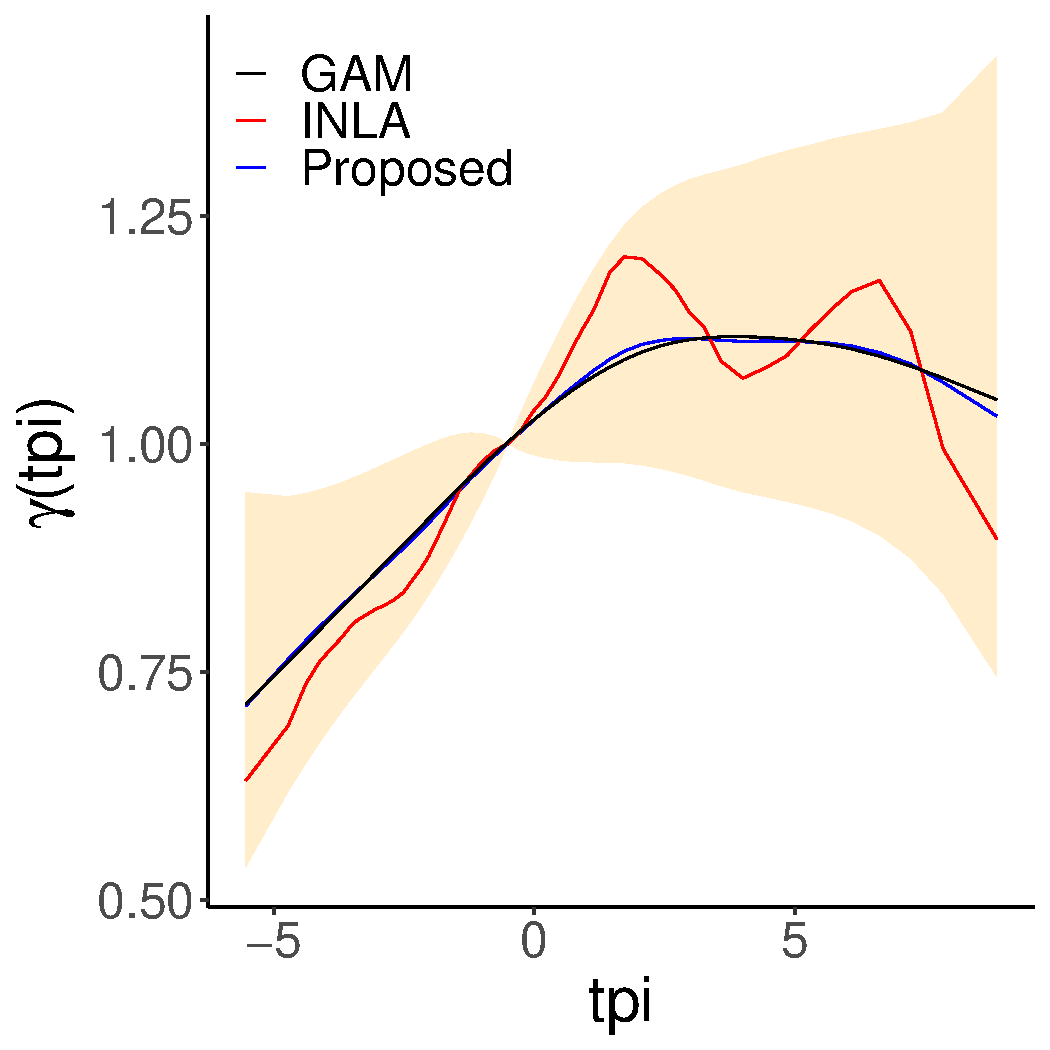
\includegraphics[width=0.45\textwidth,height=2.5in]{leuk_smooth.pdf}
}
\subcaptionbox{Posterior distribution of $\sigma$}{
	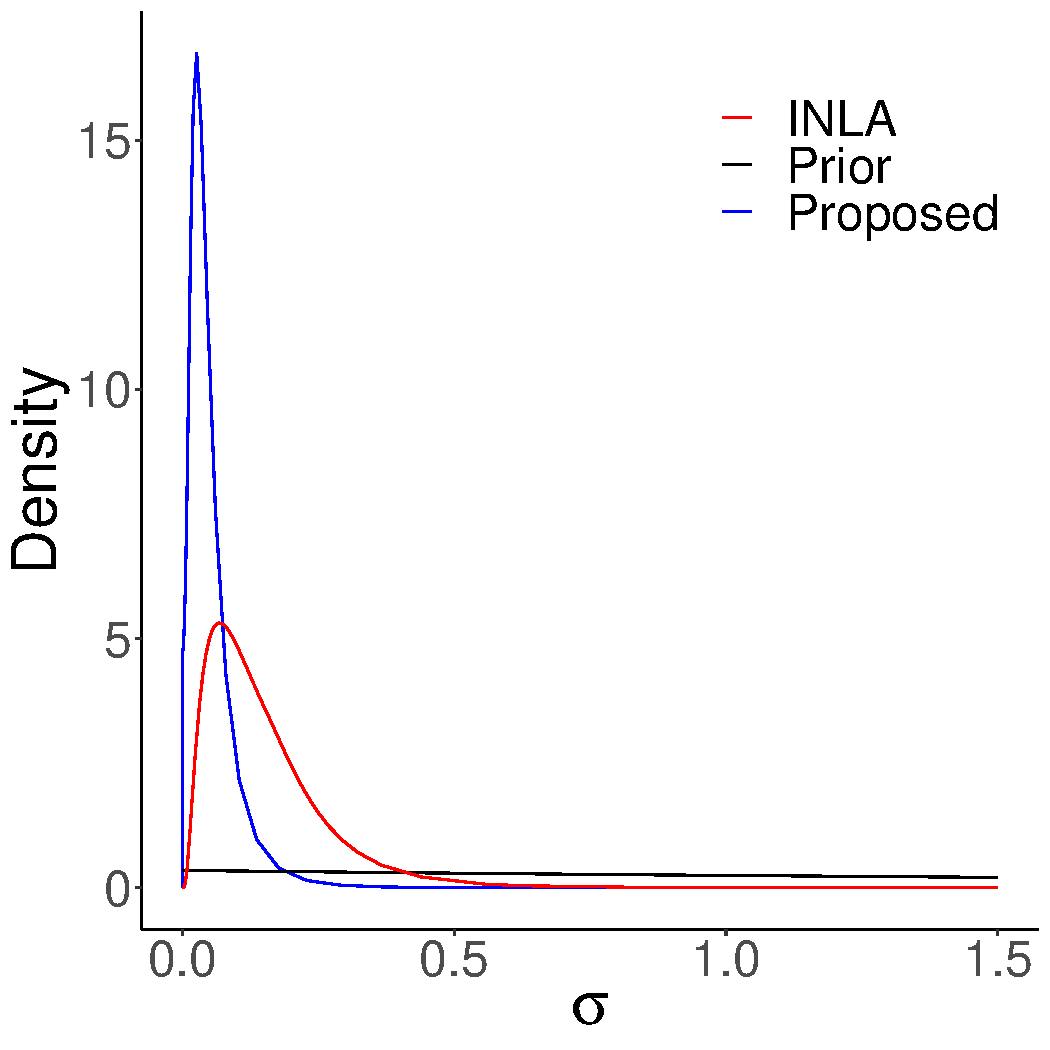
\includegraphics[width=0.45\textwidth,height=2.5in]{leuk_hyper.pdf}
}
\caption{Results for the Leukaemia data in section \ref{subsec:leuk}. (a): posterior mean (blue) and $95\%$ credible interval (shaded) using our method, posterior mean using INLA (red), and the result of fitting a GAM (black). (b): prior (black) and approximate posterior distribution for $\sigma$ using our method (blue) and INLA (red).}
\label{fig:leuk}
\end{figure}

Figure \ref{fig:leuk} shows the results of our procedure as well as those of INLA and a frequentist Generalized Additive Model (GAM). Our inferred covariate effect closely matches the point estimate returned by the GAM, however we provide full model-based posterior uncertainty for $\sigma$ where the GAM does not. The covariate effect inferred by INLA is more variable than ours, as reflected by both the shape of the posterior mean for $\Gamma_{1}$ and the width of the posterior for $\sigma_{1}$.

\subsection{Kidney Catheter Data}\label{subsec:kidney}

The Kidney Catheter dataset contains 76 times to infection, at the point of insertion of the catheter, for $n = 38$  kidney patients. Each patient $i=1,\ldots,n$ forms a group, and the time to infection of each patient's $n_{i} = 2$ kidneys represent a survival time. An observation for the survival time of a kidney is censored if the catheter is removed for reasons other than an infection. We use our procedure to fit a Cox PH model to these grouped data, providing full posterior uncertainty over the between-subject standard deviation.

We associate survival times with covariates sex, age, and indicator of one of four types of pre-existing disease each patient may have. Subject-specific intercepts $\xi_{i}\overset{iid}{\sim}\text{N}(0,\sigma^{2}_{\xi})$ are included to account for correlation between kidneys from the same subject. We use an $\text{Exponential}$ prior distribution for $\sigma_{\xi}$ with median 2.

Table \ref{table:KidneyFixed} shows the results of our procedure compared to that obtained using frequentist maximum partial likelihood methods and INLA. Our posterior means and standard deviations for the linear covariate effects are comparable to the frequentist estimates. However, as shown in Figure \ref{fig:BetweenSubjectSD}, our method provides full posterior uncertainty for $\sigma_{\xi}$ while the frequentist approach does not. INLA gives different estimates for the linear effects and reports lower posterior standard deviations. This is also reflected in Figure \ref{fig:BetweenSubjectSD}, where our posterior for $\sigma_{\xi}$ is wider than that of INLA.

\begin{figure}[ht]
\centering
\subcaptionbox{Posterior distribution of $\sigma$}{
	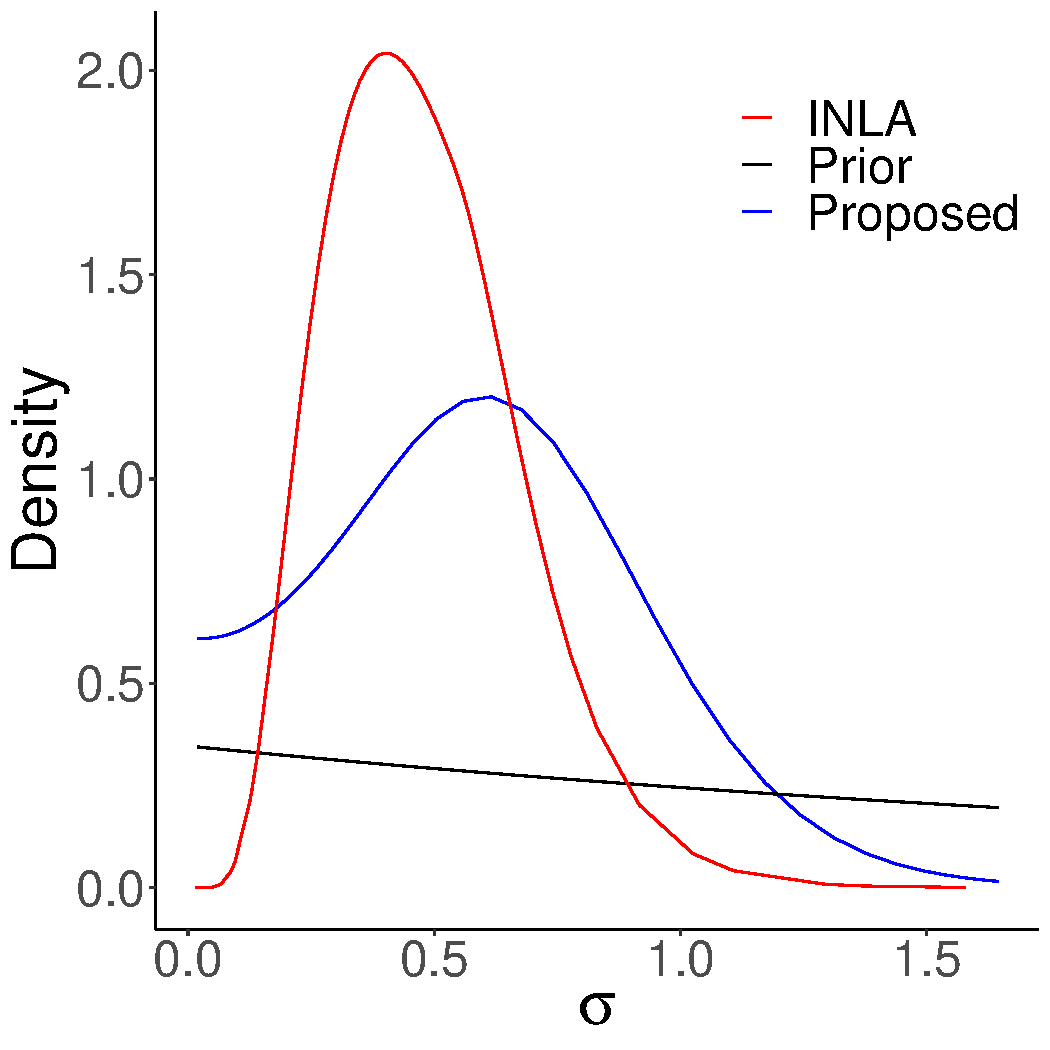
\includegraphics[width=0.45\textwidth,height=2.5in]{kidney_hyper.pdf}
}
\caption{Posterior distribution for the between-subject standard deviation by our method (blue) and by INLA (red), and its prior (black), for the kidney data in section \ref{subsec:kidney}.}
\label{fig:BetweenSubjectSD}
\end{figure}

\section{Discussion}\label{sec:discussion}

The methodology we proposed in this paper provides a flexible way to carry out Bayesian inference for Cox proportional hazard models with partial likelihood, that accommodates the inference on linear covariate effects, semi-parametric covariate effects and frailties. The use of partial likelihood does not require the smoothness assumption on the baseline hazard function, an advantage over INLA. The use of Bayesian inference provides model-based uncertainty quantification of all parameters of interest, an advantage over the frequentist Generalized Additive Model approach. We have demonstrated the advantages of our new approach over alternatives through a simulation study and two data analyses. Our proposed method is an appealing option to adopt for the analysis of time-to-event data.

One limitation of our proposed methodology is the manner in which it scales with the sample size $N$. Since the Hessian matrix in our methodology is fully dense, its number of non-zero entries increases as $O(N^{2})$. The scalability of our procedure is limited by the need to store this matrix in memory. We avoid the computation of this Hessian matrix during the optimization step by using a quasi-Newton method, however the true Hessian matrix is still required to be evaluated and stored at the maximum to compute the posterior approximations that we use.

The framework of this proposed methodology can be extended to fit more complex models, by modifying the covariance structure of the covariate with semi-parametric effect. Temporally- and spatially-correlated survival data may be analyzed through a similar procedure. Because we accommodate the dense Hessian matrix of the log-likelihood, our approach could be extended to approximate Bayesian inference for other models with a dense Hessian matrix. We leave such extensions to future work.

\section*{Data Availability Statement}
The simulated data of example 3.1 are available in the code available with this paper at the Statistics in Medicine website on Wiley Online Library.
Data for example 3.2 were obtained from R package "INLA" \cite{inla} and are freely available.
Data for example 3.3 were obtained from R package "survival" \cite{survival-package} and are freely available. 

\appendix

\section{Derivation of Precision Matrix}

In this section we give a brief derivation of the precision matrix $Q_{\theta}$ from Equation (\ref{eqn:precmat}). The derivation is similar to that of \cite{casecross} (Web Appendix C), with a different differencing matrix. The differencing matrix $D$ is:
\begin{equation}\begin{aligned}\label{eqn:D2}
D &= \begin{pmatrix}
1 & -1 & 0 & & 0 \\
1 & 0 & -1 & & 0 \\
  &    &  & \ddots  &   \\
1 &    &       & 0 & -1 \\
\end{pmatrix}
\end{aligned}\end{equation}
As described in \S\ref{sec:method} ,our model specifies:
\begin{equation*}
\Gamma|\theta \sim \text{Normal}\left( 0,\Sigma_{\Gamma}\right); \ \xi|\theta \sim \text{Normal}\left( 0,\Sigma_{\xi}\right); \ \beta \sim \text{Normal}\left( 0,\Sigma_{\beta}\right); \ \epsilon \sim \text{Normal}\left( 0,\tau^{-1}I\right)
\end{equation*}
all independent of each other unless otherwise specified. The vector of additive linear predictors can be written as $\eta = A\Gamma + B\xi + X\beta + \epsilon$ and $\Delta = D\eta$ where $D$ is defined through Equation (\ref{eqn:D2}). This gives a joint Gaussian distribution for $W|\theta$ as:
\begin{equation*}
W|\theta = \begin{pmatrix} \Delta \\ \Gamma \\ \xi \\\beta \end{pmatrix} = \begin{pmatrix} DA & DB & DX & D \\ I & 0 & 0 & 0 \\ 0 & I & 0 & 0 \\ 0 & 0 & I & 0 \\ \end{pmatrix}\begin{pmatrix}\Gamma\\ \xi \\ \beta \\ \epsilon \end{pmatrix} 
\sim \text{Normal}\left( 0,\Sigma\right)
\end{equation*}
where
\begin{equation*}
\Sigma = \begin{pmatrix}
DA\Sigma_{\Gamma}A^{T}D^{T} + DB\Sigma_{\xi}B^{T}D^{T} + DX\Sigma_{\beta}X^{T}D^{T} + \tau^{-1}DD^{T} & DA\Sigma_{\Gamma} & DB\Sigma_{\xi} & DX\Sigma_{\beta} \\
\Sigma_{\Gamma}D^{T}A^{T} & \Sigma_{\Gamma} & 0 & 0 \\
\Sigma_{\xi}D^{T}B^{T} & 0 & \Sigma_{\xi} & 0 \\
\Sigma_{\beta}D^{T}X^{T} & 0 & 0 & \Sigma_{\beta} \\
\end{pmatrix}
\end{equation*}
The precision matrix $Q(\theta) = \Sigma^{-1}$ is obtained through direct inversion.


\nocite{*}% Show all bib entries - both cited and uncited; comment this line to view only cited bib entries;
\bibliography{myrefs}%


\clearpage
\begin{table}
\centering
\resizebox{\columnwidth}{!}{%
\begin{tabular}
{|p{2.5cm}|
p{1cm}|p{1cm}p{1cm}|p{1cm}p{1cm}|p{1cm}p{1cm}|}
\cline{1-8}
      \multicolumn{1}{l}{} &
      \multicolumn{1}{l}{} &
      \multicolumn{2}{c}{Proposed} &
      \multicolumn{2}{c}{Freq PL} &
      \multicolumn{2}{c}{INLA} \\
      Variables/Reference & Levels & {Mean} & {SD} & {Mean} & {SD} & {Mean} & {SD} \\
 \hline
 Age & & 0.0048&0.015 & 0.0052&0.015 & 0.0024&0.013\\
 Sex & & -1.7&0.46  & -1.7&0.46 &  -1.6&0.38\\
 Disease Type/Other & GN & 0.17&0.53 &  0.18&0.54 & 0.11&0.47\\
  & AN & 0.39&0.53 & 0.39&0.54 & 0.52&0.47\\
  & PKD & −1.2&0.80  & −1.1&0.81 & −1.1&0.71\\
\hline
\end{tabular}
}

\caption{Estimated means and standard deviations of linear effects by proposed method, frequentist partial likelihood maximization method (Freq PL) and INLA, for the kidney data in section \ref{subsec:kidney}.}
\label{table:KidneyFixed}
\end{table}


\end{document}

